\section{点积}
两个矢量$\bb{u}$和$\bb{v}$的点积写作$\bb{u}\cdot \bb{v}$,它在物理学和几何学著作中广泛出现\footnote{当我们尝试从物理上解释点积时,需要考虑某些技术细节。 请参阅本章末尾的讨论。}。一些作者会用这样的公式来定义点积
\begin{equation}
    \bb{u}\cdot \bb{v}=\left| \bb{u} \right|\left| \bb{v} \right|\cos \theta \,\, ,  0\le \theta \le \pi \label{equ:1.8} 
\end{equation}
其中,$\theta$表示两个矢量$\bb{u}$和$\bb{v}$之间的夹角。这个定义看起来简洁有力。诶,等一下。我们只知道如何计算得到一个矢量的长度,夹角$\theta $该如何得到呢?事实上,我们没有办法,这里我们只能将式\eqref{equ:1.8}作为夹角$\theta $的定义。因此我们需要想出一个不依赖于$\theta$的,关于$\bb{u}\cdot \bb{v}$的定义。

\begin{figure}[htbp]
	\centering
	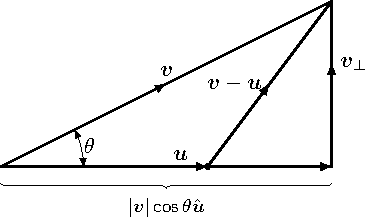
\includegraphics[width=0.4\textwidth]{./image/1.5.pdf}
	\caption{}
	\label{fig:1.5}
\end{figure}

如果$\left| \bb{u} \right|\left| \bb{v} \right| = 0$,则有$\bb{u}\cdot \bb{v}=0$。参考图\eqref{fig:1.5},一般情况下的点积定义可以用严格的几何方法来构造。图中的双向箭头反映无论两个矢量$\bb{u}$和$\bb{v}$之间的相对位置如何,夹角$\theta $恒为非负值。如图所示,矢量$\bb{v}$可以表示为矢量$\left| \bb{v} \right|\cos \theta \widehat{\bb{u}}$(它平行于$\bb{u}$)与矢量$\bb{v}_{\bot}$(它垂直于$\bb{u}$)之和。先利用两个直角三角形中较大的那一个,再利用另一个,根据勾股定理可以得到
\begin{align}
	\left| \bb{v} \right|^2&=\left| \bb{v} \right|^2\cos ^2\theta +\left| \bb{v}_{\bot} \right|^2,\label{equ:1.9}\\
	\left| \bb{v}-\bb{u} \right|^2&=\left( \left| \bb{v} \right|\cos \theta -\left| \bb{u} \right| \right) ^2+\left| \bb{v}_{\bot} \right|^2\nonumber\\
	\left| \bb{v}-\bb{u} \right|^2&=\left| \bb{v} \right|^2\cos ^2\theta -2\left| \bb{u} \right|\left| \bb{v} \right|\cos \theta +\left| \bb{u} \right|^2+\left| \bb{v}_{\bot} \right|^2\nonumber\\
	\footnotemark&=\left| \bb{u} \right|^2+\left| \bb{v} \right|^2-2\left| \bb{u} \right|\left| \bb{v} \right|\cos \theta \label{equ:1.10},
\end{align}
\footnotetext{这个结论一般被称作余弦定理。}

根据式\eqref{equ:1.9},对比式\eqref{equ:1.8}与式\eqref{equ:1.10},我们可以导出定义
\begin{equation}\label{equ:1.11}
    \bb{u}\cdot \bb{v}=\frac{1}{2}\left( \left| \bb{u} \right|^2+\left| \bb{v} \right|^2-\left| \bb{v}-\bb{u} \right|^2 \right) 
\end{equation}
注意,若$\left| \bb{u} \right|\left| \bb{v} \right| = 0$,则$\bb{u}\cdot \bb{v}=0$,这与我们用之前的定义导出的结果一致。若$\bb{u}=\bb{v}$,则
\begin{equation}
    \bb{v}\cdot \bb{v}=\left| \bb{v} \right|^2
\end{equation}
若两个矢量的点积等于0,那么这两个矢量彼此垂直。

为了用计算机计算两个矢量的点积,我们需要写出点积的分量表达式。这很简单。若$\bb{u}\sim \left( u_x,u_y,u_z \right)$ ,$\bb{v}\sim \left( v_x,v_y,v_z \right) $,则根据式\eqref{equ:1.4}以及式\eqref{equ:1.11}
\begin{equation}\label{equ:1.13}
    \bb{u}\cdot \bb{v}=u_xv_x+u_yv_y+u_zv_z
\end{equation}

假设在不改变$\bb{u}$和$\bb{v}$的情况下,我们引入另一组笛卡尔坐标系。 通常,$\bb{u}$和$\bb{v}$相对于新轴的分量会有所不同,但式\eqref{equ:1.13}的右侧会发生变化吗?作为分量乘积的每一个单项当然会变,但它们的总和不会。为什么? 因为\eqref{equ:1.11}是根据长度定义$\bb{u}\cdot \bb{v}$的,而在欧几里德几何中,长度定义不受所选坐标系的影响。因此,我们说点积是一个几何不变量。

点积的另一个关键属性是它满足分配率,也就是说
\begin{equation}\label{equ:1.14}
	\bb{u}\cdot \left( \bb{v}+\bb{w} \right) =\bb{u}\cdot \bb{v}+\bb{u}\cdot \bb{w}\,\, ,  \forall \bb{u},\bb{v},\bb{w}
\end{equation}
为了证明:式\eqref{equ:1.14},我们设$\bb{w}\sim \left( w_x,w_y,w_z \right) $。根据式\eqref{equ:1.13},则有
\begin{align*}
	\bb{u}\cdot \left( \bb{v}+\bb{w} \right) &=u_x\left( v_x+w_x \right) +u_y\left( v_y+w_y \right) +u_z\left( v_z+w_z \right)\\
	&=u_xv_x+u_yv_y+u_zv_z+u_xw_x+u_yw_y+u_zw_z\\
	&=\bb{u}\cdot \bb{v}+\bb{u}\cdot \bb{w}
\end{align*}
\qed

这个证明:的过程说明了一个很重要的问题:一般情况下,一个几何定理最适合在笛卡尔坐标系中来证明:。相应的,由于式\eqref{equ:1.14}的结论与具体的坐标系无关,因此它直接推自式\eqref{equ:1.11}。可以参考练习1.7。记住,对于一个问题,既要从几何方面思考,也要从代数方面思考,虽然可能某一种方法的证明:相较于另一种更加困难,但是也可能会带来新的思考与新的收获。

\begin{example}
若$\bb{u}\sim \left( 1,2,3 \right) $,$\bb{v}\sim \left( -3,1,-2 \right) $,计算$\bb{u}\cdot \bb{v}$的值和它们的夹角。
\end{example}
\begin{solution}
根据式\eqref{equ:1.14}
\begin{equation*}
	\bb{u}\cdot \bb{v}=\left( 1 \right) \left( -3 \right) +\left( 2 \right) \left( 1 \right) +\left( 3 \right) \left( -2 \right) =-7
\end{equation*}
并由式\eqref{equ:1.8}
\begin{equation*}
	\theta =\arccos \frac{\bb{u}\cdot \bb{v}}{\left| \bb{u} \right|\left| \bb{v} \right|}\,\, ,  0\le \theta \le \pi 
\end{equation*}
此时
\begin{align*}
	\left| \bb{u} \right|&=\sqrt{1^2+2^2+3^2}=\sqrt{14}\\
	\left| \bb{v} \right|&=\sqrt{\left( -3 \right) ^2+1^2+\left( -2 \right) ^2}=\sqrt{14}
\end{align*}
因此
\begin{equation*}
	\theta =\arccos \left( -7/14 \right) =120\degree=\frac{2}{3}\pi 
\end{equation*}
\end{solution}